\documentclass{standalone}

\usepackage{tikz}
\usetikzlibrary{matrix}

\begin{document}
  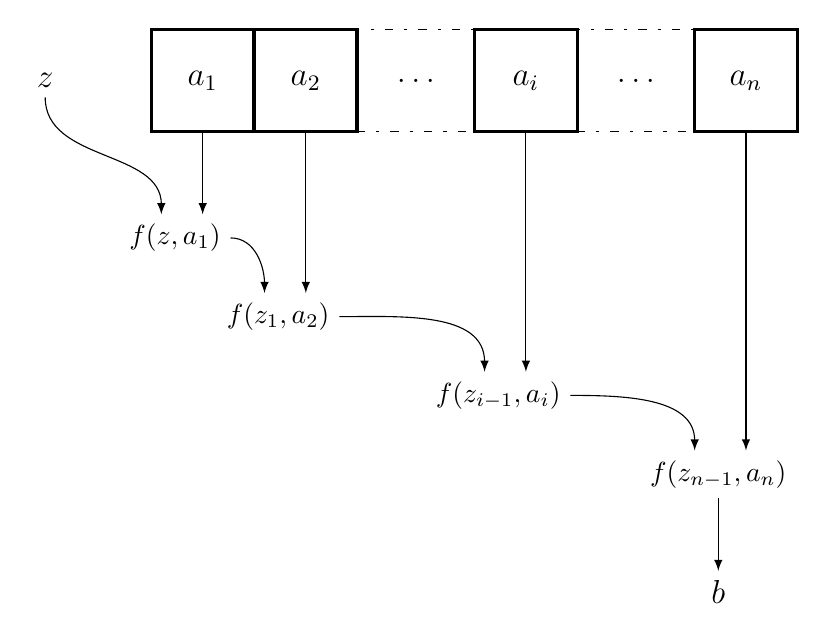
\begin{tikzpicture}

  \newcommand{\true}{\textcolor{green}{\ding{51}}}
\newcommand{\false}{\textcolor{red}{\ding{55}}}

\tikzstyle{elem}=[
  font=\large
]

\tikzstyle{cell}=[
  draw,
  line width=0.4mm,
  minimum size=1.3cm,
  outer sep=0,
  fill=white,
  font=\large
]

\tikzstyle{collection}=[
  inner sep=0,
  column sep=-0.3mm,
  nodes=cell
]

\tikzstyle{option}=[cell]

\tikzstyle{ellipsis}=[
  loosely dash dot,
  line width=0.15mm,
  minimum width=1.5cm,
  node contents=$\ldots$,
  fill=none
]

\newcommand{\ellipsis}{ \node [ellipsis]; }

\tikzstyle{tuple comma}=[
  minimum width=2em,
  draw=none,
  fill=none,
  column sep=0.3mm,
  node contents={,}
]

\newcommand{\tuplecomma}{ \node [tuple comma]; }

\tikzstyle{arrow}=[draw=black, -latex]

\tikzstyle{arrow label}=[
  font=\small,
  fill=white!0
]

\tikzstyle{white border}=[
  preaction={draw=white, line cap=butt, -, line width=0.5em},
  shorten <= 1pt,
  shorten >= 1pt
]

\tikzstyle{iteration}=[
  arrow,
  bend right=45,
  densely dashed,
  draw=gray!75
]

\tikzstyle{predicate}=[
  font=\small
]

\tikzstyle{smooth}=[
  out=270,
  in=90
]

\tikzstyle{function result}=[
  pin edge={->, decorate, decoration={snake, amplitude=0.5mm}}
]

\tikzstyle{measure}=[
  arrows={Stealth[inset=0pt, angle'=30]-Stealth[inset=0pt, angle'=30]}
]

\newcommand{\bottommeasure}[4][5mm] {
  \begin{scope}[line width=0.1mm]
    \coordinate (x) at ([yshift=-#1] #3);
    \draw (x) [measure] -- node [label={[label distance=-1mm]above:#2}] {} (x -| #4);
    \draw (#3) -- ++(0, -#1) -- +(0, -1.25mm);
    \draw (#4) -- ++(0, -#1) -- +(0, -1.25mm);
  \end{scope}
}

\newcommand{\topmeasure}[4][5mm] {
  \begin{scope}[line width=0.1mm]
    \coordinate (x) at ([yshift=#1] #3);
    \draw (x) [measure] -- node [label={[label distance=-1mm]above:#2}] {} (x -| #4);
    \draw (#3) -- ++(0, #1) -- +(0, 1.25mm);
    \draw (#4) -- ++(0, #1) -- +(0, 1.25mm);
  \end{scope}
}

\tikzstyle{bottombrace}=[
  decorate, decoration={brace, amplitude=1mm, raise=1mm, mirror}
]
\tikzstyle{topbrace}=[
  decorate, decoration={brace, amplitude=1mm, raise=1mm}
]
\tikzstyle{from brace}=[shorten <=2mm]
\tikzstyle{to brace}=[shorten >=2mm]

\newcommand{\bracetobrace}[4] {
  \coordinate (a) at (#1);
  \coordinate (b) at (#2);
  \coordinate (c) at (#3);
  \coordinate (d) at (#4);
  \draw [bottombrace] (a) -- coordinate (e) (b);
  \draw [topbrace] (c) -- coordinate (f) (d);
  \draw [from brace, to brace, arrow] (e) -- (f);
}

\newcommand{\toppointer}[2] {
  \draw ([yshift=1mm] #1) [Latex-] -- ([yshift=1cm] #1) node [anchor=south] {#2};
}



\matrix (A) [collection, name prefix=a] {
    \node (1) {$a_1$}; &
    \node (2) {$a_2$}; &
    \ellipsis          &
    \node (i) {$a_i$}; &
    \ellipsis          &
    \node (n) {$a_n$}; \\
};

\node (z) [elem, left of=a1, node distance=2cm] {$z$};

\foreach \i/\z [count=\c] in {1/z,2/z_1,i/z_{i-1},n/z_{n-1}} {
  \node (f\i) [below of=a\i, node distance={1cm + \c * 1cm}, xshift=-1em] {$f(\z, a_{\i})$};
  \draw (a\i) [arrow] to (a\i |- f\i.north);
}

\node (B) [elem, below of=fn, node distance=1.5cm] {$b$};

\draw [arrow, out=270, in=90] (z.south) to (f1.120);
\draw [arrow, out=0, in=90] (f1.east) to (f2.120);
\draw [arrow, out=0, in=90] (f2.east) to (fi.120);
\draw [arrow, out=0, in=90] (fi.east) to (fn.135);
\draw [arrow] (fn.south) -- (B.north);

  \end{tikzpicture}
\end{document}

